\scnheader{Программный вариант реализации платформы интерпретации sc-моделей компьютерных систем}
\scntext{принципы реализации}{Поскольку sc-тексты представляют собой семантические сети, то есть, по сути, графовые конструкции определенного вида, то на нижнем уровне задача разработки программного варианта реализации платформы интерпретации sc-моделей сводится к разработке средств хранения и обработки таких графовых конструкций.

К настоящему времени разработано большое количество простейших моделей представления графовых конструкций в линейной памяти, таких как матрицы смежности, списки смежности и другие (\scncite{Diskrete_Math}). Однако, при разработке сложных систем как правило приходится использовать более эффективные модели, как с точки зрения объема информации, требуемого для представления, так и с точки зрения эффективности обработки графовых конструкций, хранимых в той или иной форме.

К наиболее распространенным программным средствам, ориентированным на хранение и обработку графовых конструкций относятся графовые СУБД (Neo4j \scncite{Neo4j}, ArangoDB \scncite{ArangoDB}, OrientDB \scncite{OrientDB}, Grakn \scncite{Grakn} и др.), а также так называемые rdf-хранилища (Virtuoso \scncite{Virtuoso}, Sesame \scncite{Sesame} и др.), предназначенные для хранения конструкций, представленных в модели RDF. Для доступа к информации, хранимой в рамках таких средств, могут использоваться как языки, реализуемые в рамках конкретного средства (например, язык Cypher в Neo4j), так и языки, являющиеся стандартами для большого числа систем такого класса (например, SPARQL для rdf-хранилищ).

Популярность и развитость такого рода средств приводит к тому, что на первый взгляд целесообразным и эффективным кажется вариант реализации \textit{программного варианта реализации платформы интерпретации sc-моделей} на базе одного из таких средств. Однако, существует ряд причин, по которым было принято решение о реализации \textit{программного варианта реализации платформы интерпретации sc-моделей} с нуля. К ним относятся следующие:

    \begin{scnitemize}
        \item для обеспечения эффективности хранения и обработки информационных конструкций определенного вида (в данном случае -- конструкций SC-кода, sc-конструкций), должна учитываться специфика этих конструкций. В частности, описанные в работе \scncite{Koronchik2013} эксперименты показали значительный прирост эффективности собственного решения по сравнению с существующими на тот момент;
        \item в отличие от классических графовых конструкций, где дуга или ребро могут быть инцидентны только вершине графа (это справедливо и для rdf-графов) в SC-коде вполне типичной является ситуация, когда sc-коннектор инцидентен другому sc-коннектору или даже двум sc-коннекторам. В связи с этим существующие средства хранения графовых конструкций не позволяют в явном виде хранить sc-конструкции (sc-графы). Возможным решением данной проблемы является переход от sc-графа к орграфу инцидентности, пример которого описан в работе \scncite{Ivashenko2015}, однако такой вариант приводит к увеличению числа хранимых элементов в несколько раз и значительно снижает эффективность алгоритмов поиска из-за необходимости делать большое количество дополнительных итераций;
        \item в основе обработки информации в рамках Технологии OSTIS лежит многоагентный подход, в рамках которого агенты обработки информации, хранимой в sc-памяти (sc-агенты) реагируют на события, происходящие в sc-памяти и обмениваются информацией посредством спецификации выполняемых ими действий в sc-памяти \scncite{Shunkevich2018}. В связи с этим одной из важнейших задач является реализация в рамках \textit{программного варианта реализации платформы интерпретации sc-моделей} возможности подписки на события, происходящие в программной модели sc-памяти, которая на данный момент практически не поддерживается в рамках современных средств хранения и обработки графовых конструкций;
        \item SC-код позволяет описывать также внешние информационные конструкции любого рода (изображения, текстовые файла, аудио- и видеофайлы и т.д.), которые формально трактуются как содержимое \textit{sc-элементов}, являющихся знаками \textit{внешних файлов ostis-системы}. Таким образом, компонентом \textit{программного варианта реализации платформы интерпретации sc-моделей} должна быть реализация файловой памяти, которая позволяет хранить указанные конструкции в каких-либо общепринятых форматах. Реализация такого компонента в рамках современных средств хранения и обработки графовых конструкций также не всегда представляется возможной.
    \end{scnitemize}

    По совокупности перечисленных причин было принято решение о реализации \textit{программного варианта реализации платформы интерпретации sc-моделей} "с нуля"{} с учетом особенностей хранения и обработки информации в рамках Технологии OSTIS.}
\scnrelfromset{декомпозиция программной системы}{Программная модель sc-памяти;Реализация интерпретатора sc-моделей пользовательских интерфейсов}
\scnexplanation{Текущий \textit{Программный вариант реализации платформы интерпретации sc-моделей компьютерных систем} является web-ориентированным, то есть с точки зрения современной архитектуры каждая \mbox{ostis-система} представляет собой web-сайт доступный онлайн посредством обычного браузера. Такой вариант реализации обладает очевидным преимуществом -- доступ к системе возможен из любой точки мира, где есть Интернет, при этом для работы с системой не требуется никакого специализированного программного обеспечения. С другой стороны, такой вариант реализации обеспечивает возможность параллельной работы с системой нескольких пользователей.

В то же время, взаимодействие клиентской и серверной части организовано таким образом, что \mbox{web-интерфейс} может быть легко заменен на настольный или мобильный интерфейс, как универсальный, так и специализированный.

Данный вариант реализации распространяется под open-source лицензией, для хранения исходных текстов используется хостинг Github и коллективная учетная запись ostis-ai.

Реализация является кроссплатформенной и может быть собрана из исходных текстов в различных операционных системах.}
\scnrelfrom{иллюстрация}{\scnfileimage{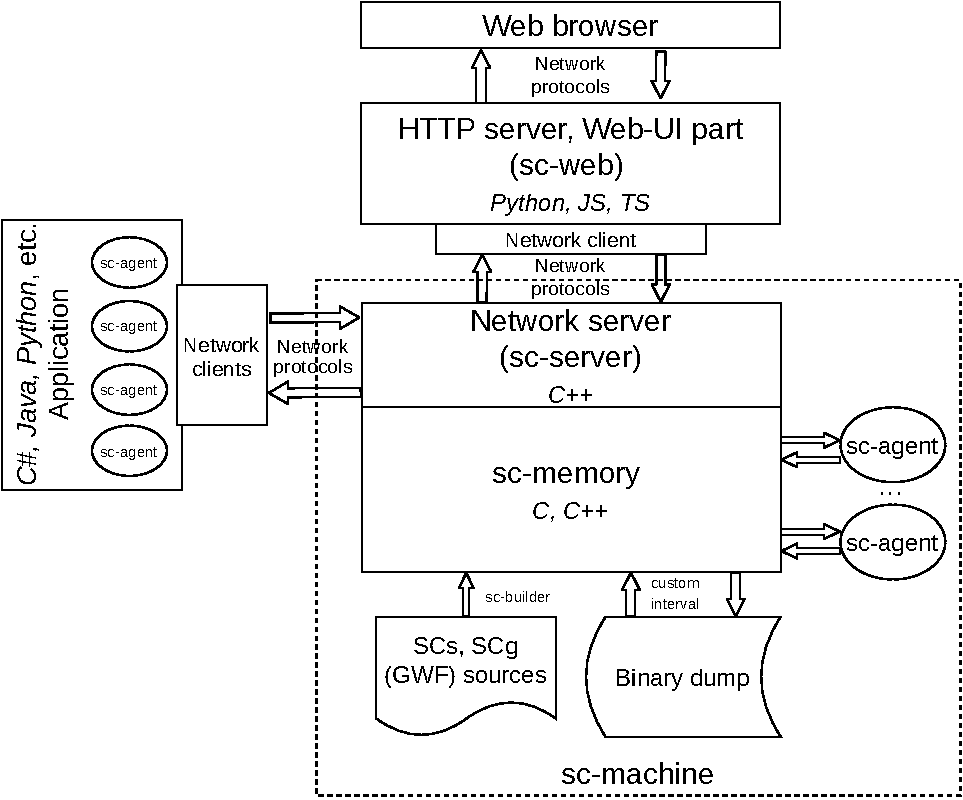
\includegraphics[scale=0.95]{../docs/images/platform_arch}}}
\scnaddlevel{1}
\scnexplanation{На приведенной иллюстрации видно, что ядром платформы является \textit{Программная модель sc-памяти} (sc-machine), которая одновременно может взаимодействовать как с \textit{Реализацией интерпретатора sc-моделей пользовательских интерфейсов} (sc-web \scncite{sc_web}), так и с любыми сторонними приложениями по соответствующим сетевым протоколам. С точки зрения общей архитектуры \textit{Реализация интерпретатора sc-моделей пользовательских интерфейсов} выступает как один из множества возможных внешних компонентов, взаимодействующих с \textit{Программной моделью sc-памяти} по сети.}
\scnaddlevel{-1}

\subimport{../sc-machine/docs/}{sc_machine}
\subimport{../sc-web/docs/}{sc_web}
